% Generated from validated hardened stage artifacts.

\section{Engineered calibration and held-out trained-readout assays}

\paragraph{Known-mechanism calibration.}

Oracle motif features implanted in QK and V span TATA and CTCF, single-head, query-specific, distributed, composition-only, and randomized computations. Strength, position, and instance count vary. Thresholds chosen on discovery seeds yield confirmation sensitivity 1.000 and false-positive rate 0.000. This validates engineered base-token fixtures, not sensitivity to learned DNABERT mechanisms.

\begin{figure}[t]\centering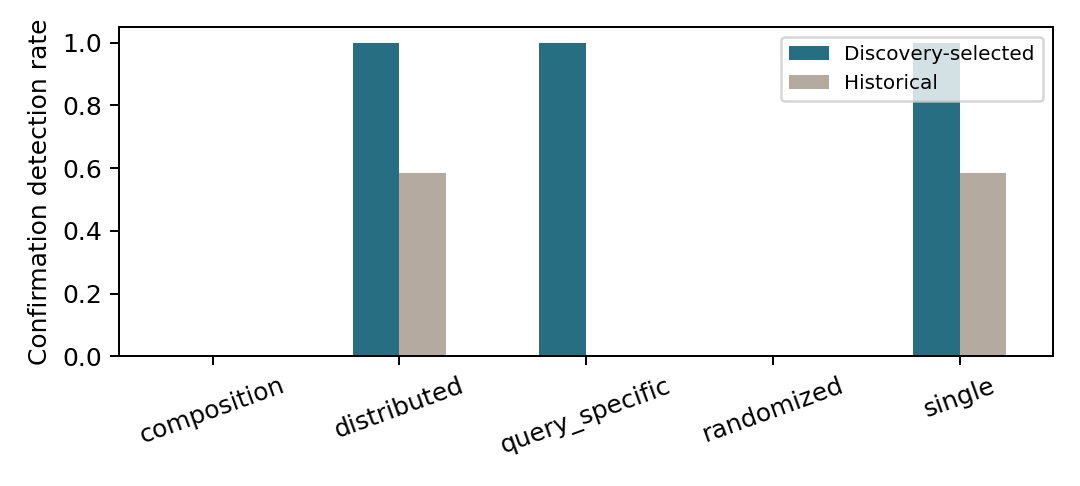
\includegraphics[width=.85\linewidth]{../results/hardened/figures/calibration.png}\caption{Oracle fixture calibration on separate fixture seeds; per-observation head selection does not calibrate natural-data selection.}\end{figure}

\paragraph{Incremental prediction.}

Baseline features include mono- and dinucleotide composition, motif count, score and relative position, and window coordinates. Baseline-only and baseline-plus-residual models use identical populations, validation-selected regularization, and fixed held-out predictions. Table~\ref{tab:incremental} gives paired 1 Mb genomic-block intervals.

\begin{table}[t]\centering\normalsize\caption{Baseline-plus-residual minus baseline-only AUROC.}\label{tab:incremental}

\begin{tabular}{lrrr}
\toprule
Task & $\Delta$ AUROC & 95\% block interval & Clusters \\
\midrule
TATA & 0.0412 & [0.0111, 0.0678] & 87 \\
Other promoter & 0.0240 & [0.0137, 0.0352] & 107 \\
Donor & 0.2089 & [0.1814, 0.2385] & 107 \\
Acceptor & 0.2360 & [0.2024, 0.2670] & 107 \\
Accessible CTCF & -0.0454 & [-0.0756, -0.0166] & 81 \\
\bottomrule
\end{tabular}

\end{table}

\paragraph{Aligned composition controls.}

Motif and sham edits preserve exact A/C/G/T counts and match nucleotide transitions, edit count, window width, overlapping BPE count, and covered nucleotide width. Shams occupy the nearest eligible non-motif window, with distance logged. All token boundaries agree, the target motif is destroyed, and no new threshold-passing hit locations are created. Eligibility uses sequence properties without output filtering. Six of ten historical TATA pairs have incompatible boundaries at patched positions; their PM rankings are withdrawn as aligned intervention evidence.

Discovery on chromosomes 18/19 chooses one of 144 heads, whose identity and scorer are frozen before confirmation on 20/21. Absolute motif-minus-sham score changes are primary. Edits are averaged within sequence; genomic blocks merge shared intervals and exact or reverse-complement inputs. Discovery carries simultaneous maximum-statistic inference. Confirmation saves individual scores, leave-one-out estimates, and six schemes in both denoising and reverse directions. The original secondary column used sequence Holm. Reporting revision v1 below supplies both dependence units; block Holm governs block-based interpretation. Donor GT edits retain insufficient aligned matched examples, so no donor mechanism is inferred.

\begin{table}[t]\centering\normalsize\caption{Fixed-head trained-readout intervention on held-out chromosomes.}\label{tab:controlled}

\begin{tabular}{lrrrrr}
\toprule
Motif & Head & Sequences & Effect & 95\% block interval & $p$ \\
\midrule
TATA & 0/8 & 16 & 0.0243 & [-0.0338, 0.1014] & 0.5772 \\
CTCF & 5/8 & 64 & 0.0157 & [0.0066, 0.0251] & 0.0028 \\
\bottomrule
\end{tabular}

\end{table}

\begin{figure}[t]\centering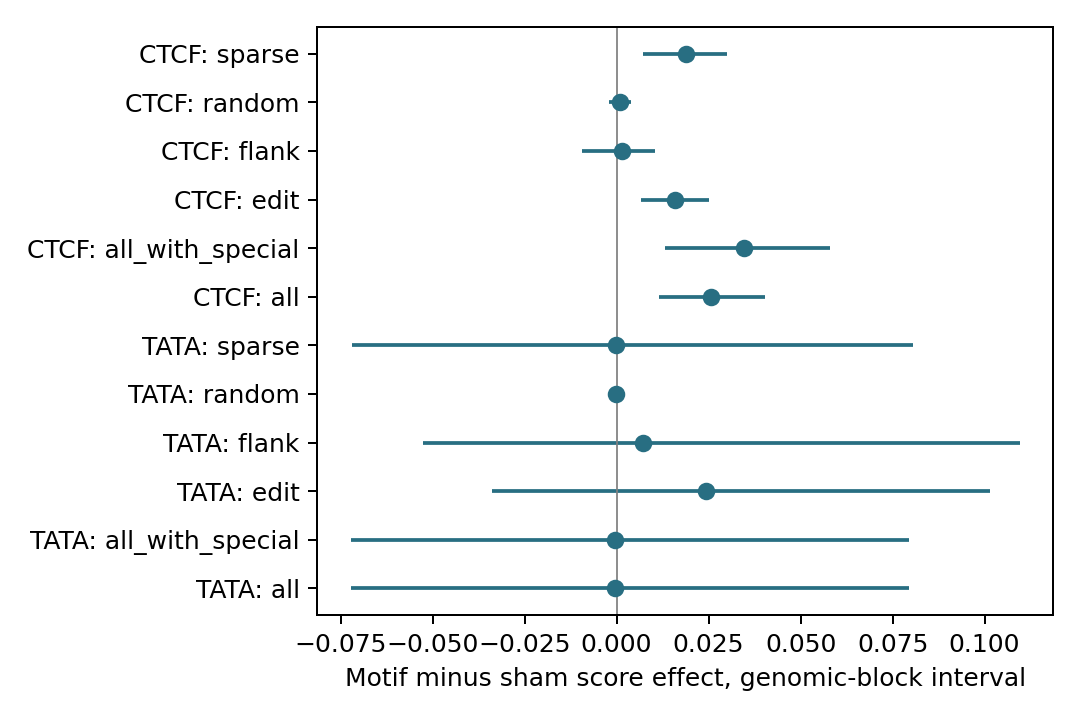
\includegraphics[width=.9\linewidth]{../results/hardened/figures/controlled_interventions.png}\caption{Genomic-block intervals for fixed-head denoising schemes; secondary schemes are exploratory.}\end{figure}

\paragraph{Independent accessible CTCF cohort.}

GM12878 DNase experiment ENCSR000EMT, GRCh38 file ENCFF598KWZ, defines accessible windows independently of the saved CTCF peaks. Cases overlap those peaks; controls do not, including motif-bearing non-overlap windows. Matching uses chromosome, 204 bp width, GC within 0.02, and log-DNase signal within 0.5. Per-class caps are 512 training, 128 validation, and 128 test. The readout passes its pre-execution validation AUROC gate of 0.6 with validation AUROC 0.6859 and test AUROC 0.6699. Localization and intervention use the same CTCF motif and trained output. The paired incremental comparison in Table~\ref{tab:incremental} is negative for CTCF: this fitted concatenation underperforms the fitted direct baseline, without establishing absence of extra representational information. Peak non-overlap does not verify binding absence. Repeat annotations, quantitative occupancy, and other cell types are unavailable.

\paragraph{Native attention sensitivity.}

PWM score-range fractions 0.7, 0.8, and 0.9 recompute scoring and matching across 51,249 peaks. Each configuration evaluates at most 256 random eligible pairs. Token balancing requires identical real-token and target-token counts and covered widths within 2 bp. Maximum, mean, and overlap-weighted aggregation give separate QK assays. Attention compares base and token weighting, global and local queries, and native, content-only, and position-only softmax. Every native head context is checked. Table~\ref{tab:geometry} counts positive base-density contrasts passing genomic-block maximum-statistic tests over 144 heads; saved inference also corrects across all sensitivity choices and reports chromosome effects.

\begin{table}[t]\centering\caption{Sensitivity counts under both saved families. Within uses 144-head maximum-statistic tests; overall Holm includes all metrics, thresholds, geometries, heads and both resampling summaries.}\label{tab:geometry}\begin{tabular}{lrrrrr}
\toprule
Fraction & Geometry & Eligible & Scored & Within & Overall \\
\midrule
0.70 & nucleotide\_matched & 82 & 82 & 0 & 0 \\
0.70 & token\_balanced & 15 & 15 & 1 & 0 \\
0.80 & nucleotide\_matched & 5220 & 256 & 7 & 0 \\
0.80 & token\_balanced & 3510 & 256 & 44 & 0 \\
0.90 & nucleotide\_matched & 13090 & 256 & 12 & 0 \\
0.90 & token\_balanced & 5088 & 256 & 55 & 0 \\
\bottomrule
\end{tabular}\end{table}

\paragraph{Scope and reproducibility.}

These experiments test computational calibration and trained-readout effects without establishing native pretrained binding causality. Protocol choices precede execution without external registration. Distant homology, label reconstruction, pretraining exposure, and classifier-seed variability remain unresolved. Immutable legacy-pipeline receipts reject changed scientific configuration, source, membership, or artifacts on resume. Isolated execution records retain prior receipts and verify source and artifact hashes before generating these results.
